% !TeX root = ../../main.tex

For a finite point set $P\subset D$ recall that the \Cech complex $\cech^\e(P)$ is defined to be the Nerve of the open cover $\{\ball_D^\e(p)\}_{p\in P}$.
When $\varrho_D > \e$ this cover is good, and the Nerve Theorem states that $\cech^\e(P)$ is homotopy equivalent to $P^\e$.
That is, we have an isomorphism $\N_w^{\e, k} : \hom_k(\cech^\e(P,Q_w))\to \hom_k(P^\e, Q_w^\e)$ on homology groups that is induced by this homotopy equivalence.% (see Appendix~\ref{apx:nerves}).

\paragraph{Duality}

The statement of Theorem~\ref{thm:geo_tcc} is in terms of the $0$-dimensional homology of complement spaces makes it difficult, if not impossible, to compute directly.
The following lemma applies a version of duality in (co)homology (see Lemma~\ref{cor:alexander_iso}, Appendix~\ref{apx:duality}) which equates the $0$-dimensional homology of complements with the $d$-dimensional homology of cover.
This is then combined with isomorphisms provided by the Nerve Theorem in order to give us a computable alternative to the hypothesis of Theorem~\ref{thm:geo_tcc}.

\begin{lemma}\label{lem:duality_apply}
  Let $\X$ be an orientable $d$-manifold let $D$ be a compact subset of $\X$ with strong convexity radius $\varrho_D > \e$.
  Let $P$ be a finite subset of $D$ such that $P^\e\subset \intr_\X(D)$ and $Q\subseteq P$.

  If $D\setminus Q^\e$ and $D\setminus P^\e$ are locally path connected then there is an isomorphism
  \[ \xi\N : \hom_d(\cech^\e(P,Q))\to \hom_0(D\setminus Q^\e, D\setminus P^\e)\]
  that commutes with maps induced by inclusions.
\end{lemma}
\begin{proof}
  Because $Q^\e$ and $P^\e$ are open in $D$ and $D$ is compact in $\X$ the complement $D\setminus Q^\e$ is closed in $D$, and therefore compact in $\X$.
  Moreover, because $P^\e\subset \intr_\X(D)$, $\hom_d(\X\setminus(D\setminus P^\e), \X\setminus(D\setminus Q^\e)) = \hom_d(P^\e, Q^\e)$.
  As we have assumed these complements are locally path connected by assumption we have a natural isomorphism $\xi : \hom_d(P^\e, Q^\e)\to \hom_0(D\setminus Q^\e, D\setminus P^\e)$
  by Lemma~\ref{cor:alexander_iso}.

  Because $\e > \varrho_D$ the covers by metric balls associated with $P^\e$ and $Q^\e$ are good, so we have isomorphisms $\N : \hom_d(\cech^\e(P, Q))\to \hom_d(P^\e, Q^\e)$ for all $Q\subseteq P$ by the Nerve Theorem.
  So the composition $\xi\N := \xi\circ\N$ is an isomorphism.
  Moreover, because $\xi$ is natural and $\N$ commutes with maps induced by inclusions by the persistent nerve lemma the composition $\xi\N$ does as well.
\end{proof}

The requirement that our complements are locally path connected is necessary in order to satisfy the general statement of the duality theorem.
A rigorous investigation of the minimal assumptions that can be made on $\X$ and $D$ is beyond the scope of this paper.
We note that, in practice, it likely suffices to assume that there exists a triangulation of $P^\e$ that is a subcomplex of some refinement of a triangulation of $\X$ (see~\cite{cavanna2017when},~\cite{julian83alexander}).

\paragraph{Assumption 2}

In order obtain an upper bound on $\rk~j$ we introduce our second assumption: that $\hom_0(D\setminus B_\omega\hookrightarrow D\setminus B_{\omega-c(\delta+\zeta)})$ is \emph{injective}---as we move away from $\omega$ moving \emph{down} no components \emph{disappear}.
Once again, in terms of $\omega$ as a super-levelset monotonically decreasing, no components \emph{disappear} right \emph{after} $\omega$.
Once again, for a function in two dimensions, this translates to features in dimension 1 appearing before $\omega$ is the sub-levelset filtration, as shown in Figure~\ref{fig:assumption2}.
% Once again, in terms of $\omega$ as a sub-levelset monotonically increasing, no components \emph{appear} right \emph{before} $\omega$.

% \begin{figure}[htbp]\label{fig:assumption_2}
%   \centering
%   % 
\includegraphics[trim=50 190 0 200, clip, scale=0.2]{scripts/figures/scalar.png}
%   % 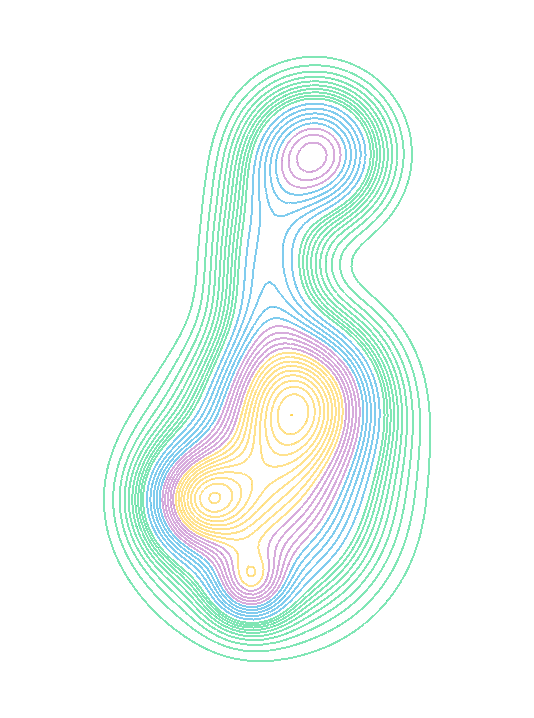
\includegraphics[trim=100 25 75 0, clip, angle=280, scale=0.25]{scripts/figures/scalar_contour.png}
%   
\includegraphics[trim=200 325 150 300, clip, scale=0.3]{scripts/figures/scalar_a2_B.png}
%   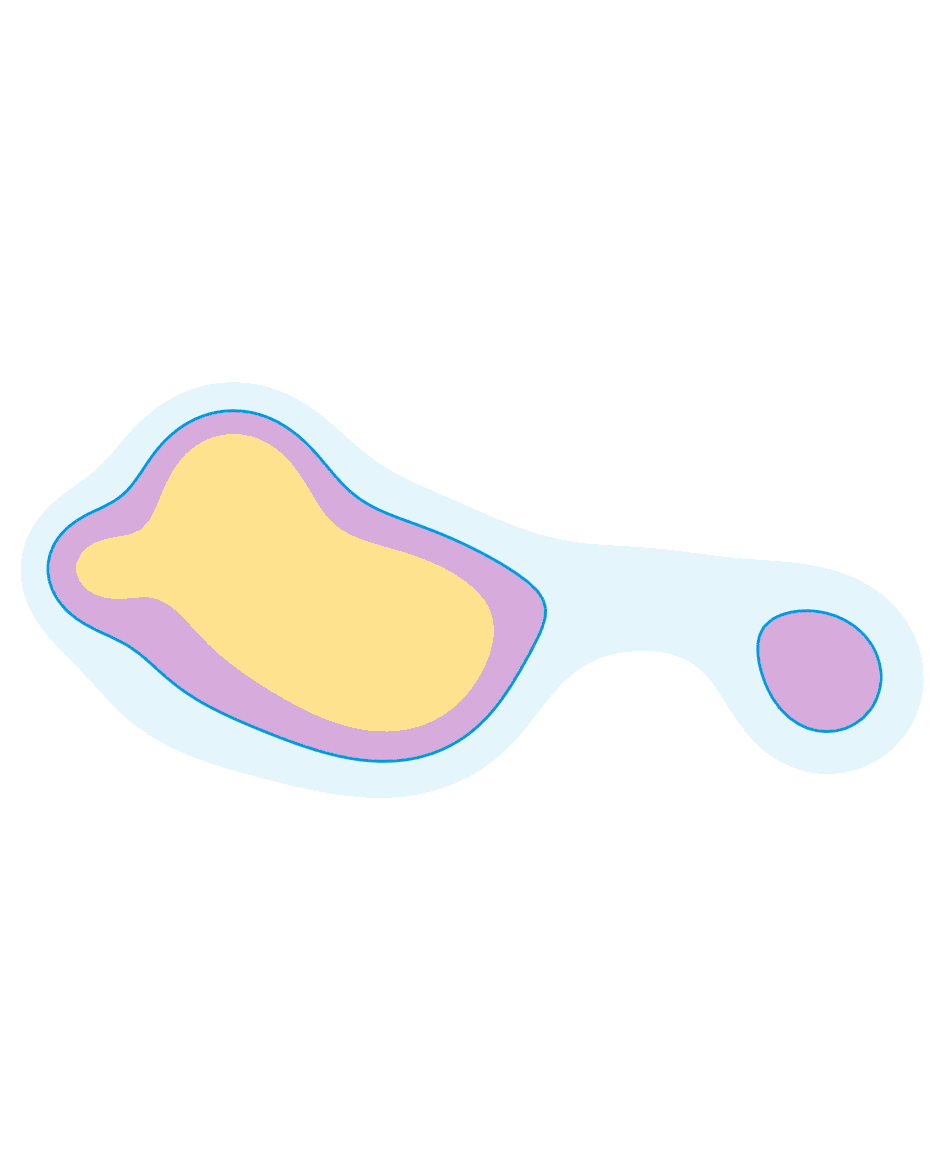
\includegraphics[trim=0 350 0 370, clip, scale=0.2]{scripts/figures/scalar_a2_B_top.png}
%   
\includegraphics[trim=200 325 150 300, clip, scale=0.3]{scripts/figures/scalar_a2_A.png}
%   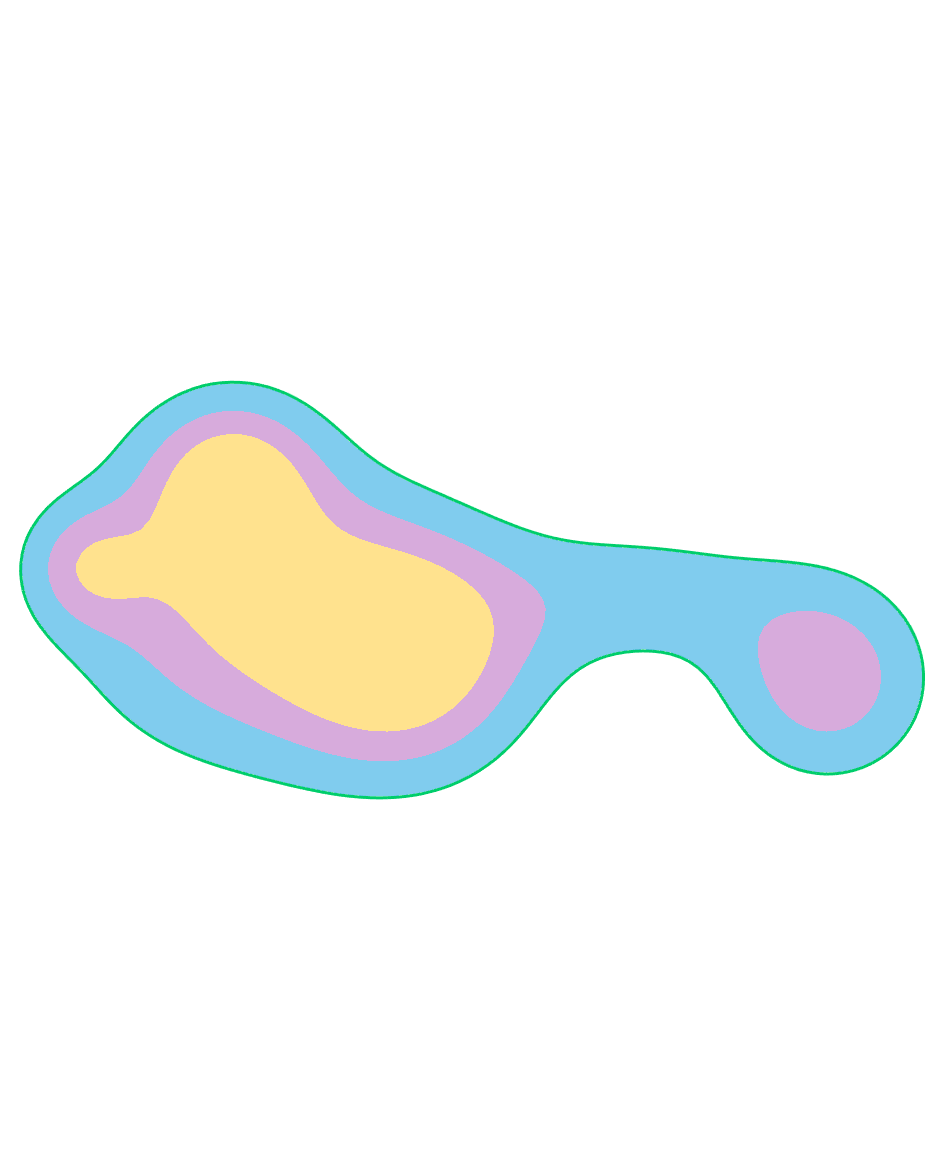
\includegraphics[trim=0 350 0 370, clip, scale=0.2]{scripts/figures/scalar_a2_A_top.png}
%   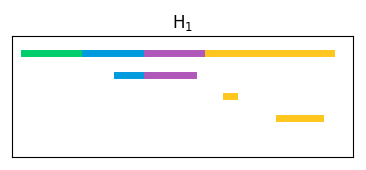
\includegraphics[scale=0.7]{scripts/figures/scalar_barcode_H1.png}
%   % \includegraphics[scale=0.55]{scripts/figures/scalar_barcode_super_0.png}
%   % \includegraphics[scale=0.55]{scripts/figures/scalar_barcode_sub_1.png}
%   \caption{\textbf{(Assumption 2)} The blue levelset does not satisfy Assumption 2 as the smaller component is not in the inclusion from blue to green.
%           This can be seen in the second feature of the barcode shown as a feature which is born in the blue region.}
% \end{figure}

\begin{figure}[htbp]\label{fig:assumption2}
  \centering
  % 
\includegraphics[trim=50 190 0 200, clip, scale=0.2]{scripts/figures/scalar.png}
  % 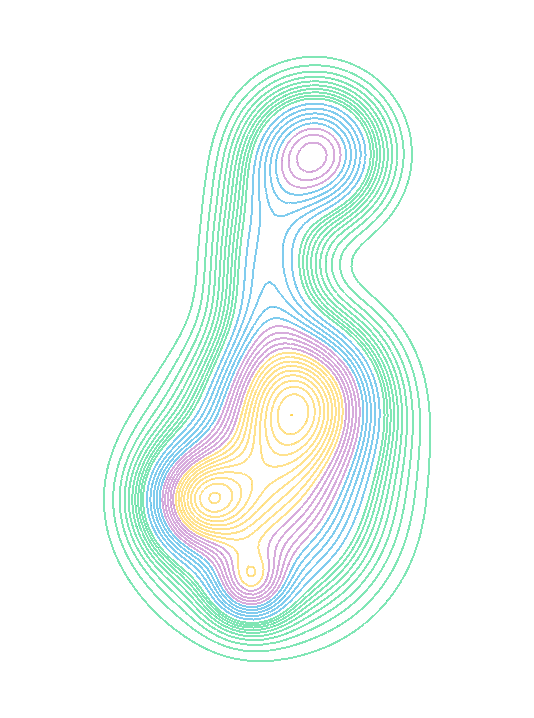
\includegraphics[trim=100 25 75 0, clip, angle=280, scale=0.25]{scripts/figures/scalar_contour.png}
  
\includegraphics[trim=200 300 200 200, clip, width=0.5\textwidth]{scripts/figures/surf/ass2_C_side.png}
  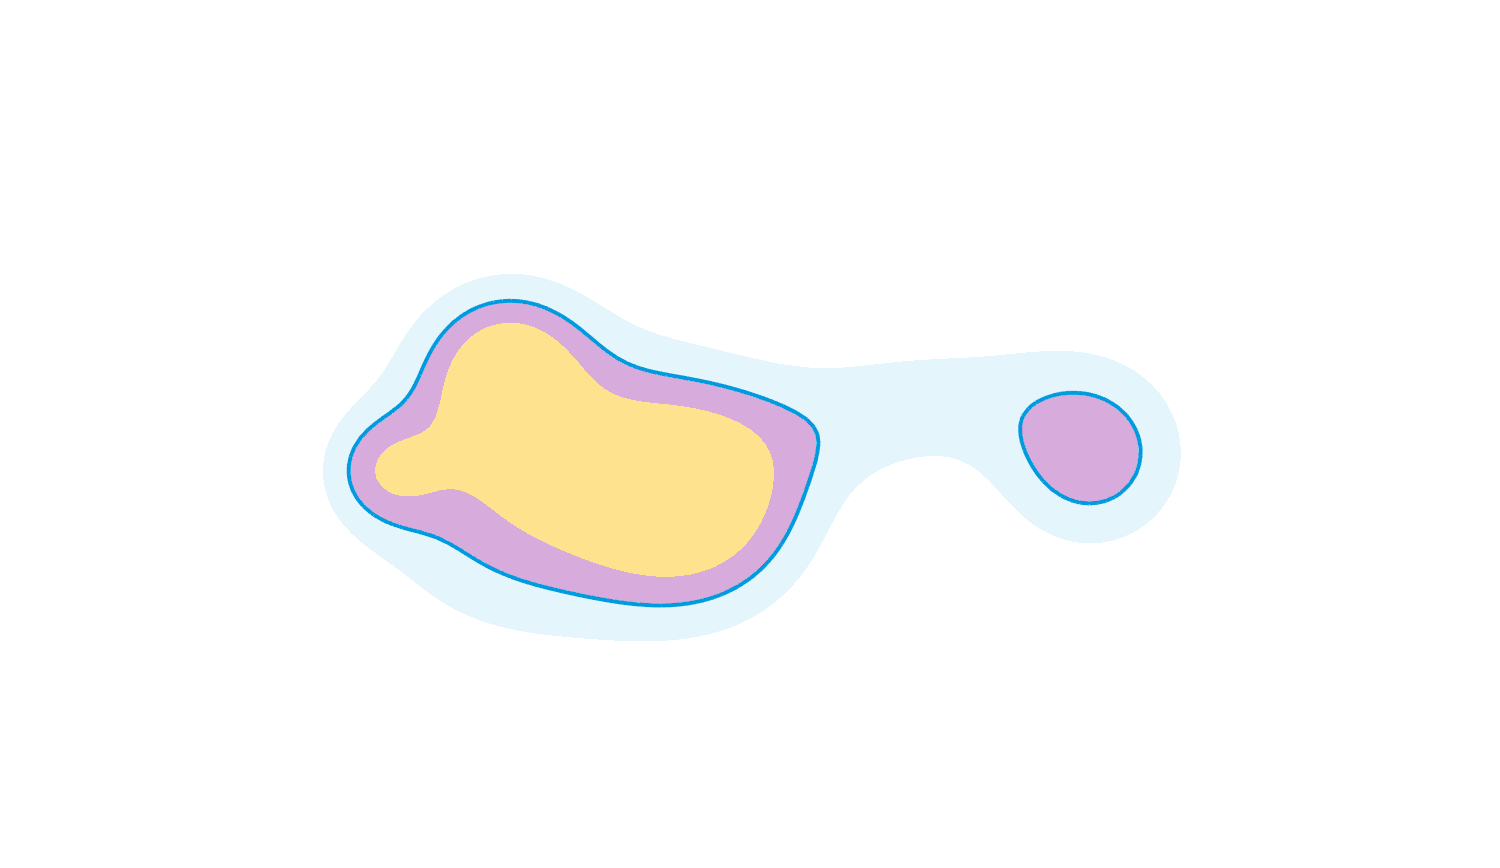
\includegraphics[trim=300 200 200 200, clip, width=0.3\textwidth]{scripts/figures/surf/ass2_C_top.png}
  
\includegraphics[trim=200 300 200 200, clip, width=0.5\textwidth]{scripts/figures/surf/ass2_B_side.png}
  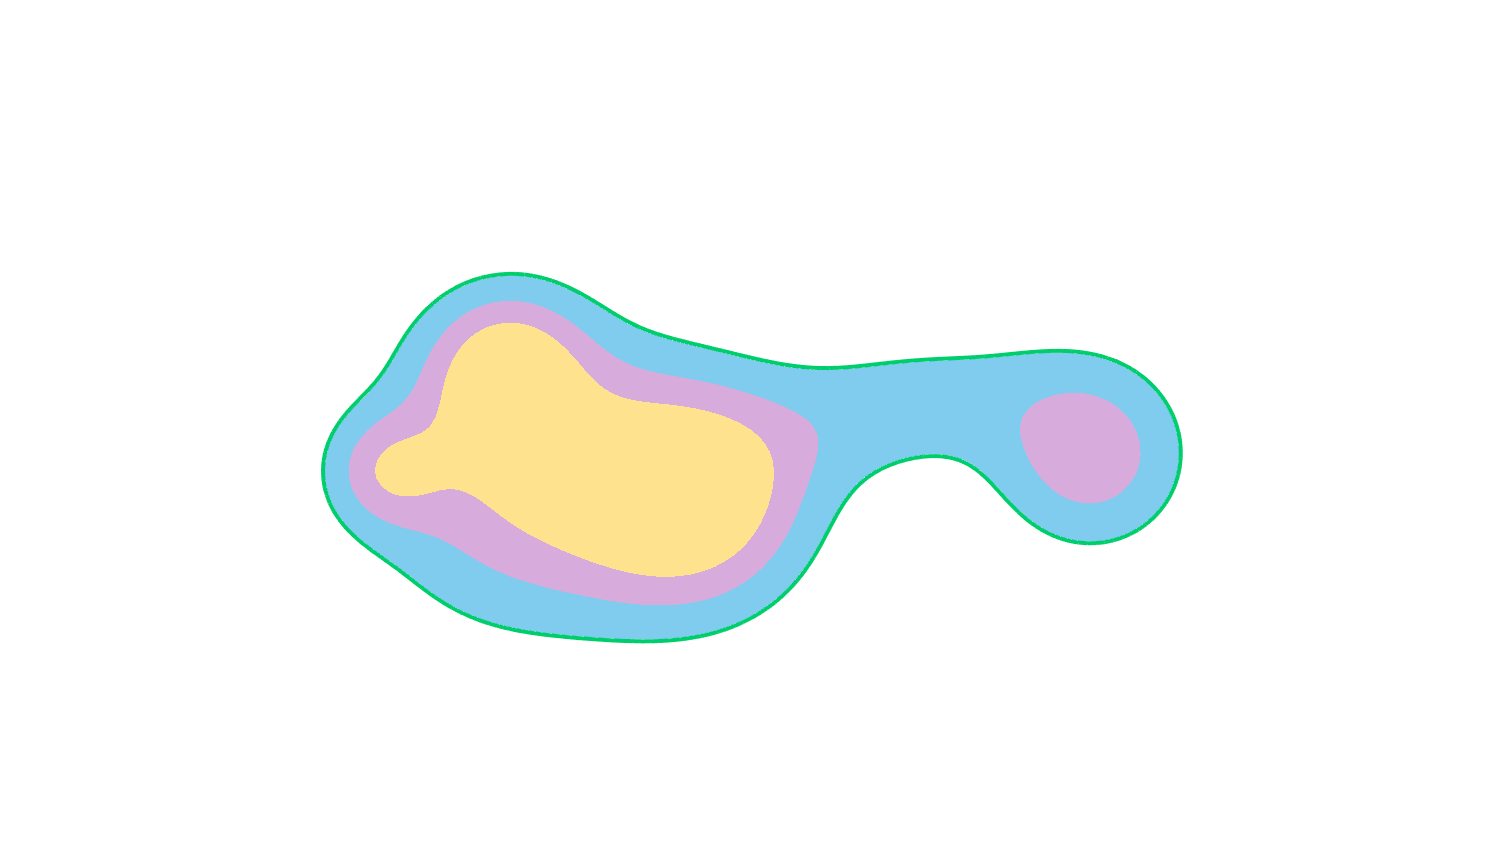
\includegraphics[trim=300 200 200 200, clip, width=0.3\textwidth]{scripts/figures/surf/ass2_B_top.png}
  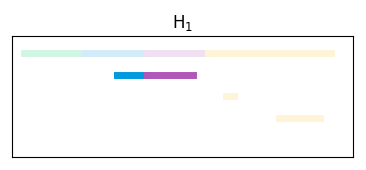
\includegraphics[scale=0.7]{scripts/figures/scalar_barcode_H1-masked.png}
  \caption{\textbf{(Assumption 2)} The blue levelset does not satisfy Assumption 2 as the smaller component is not in the inclusion from blue to green.
          This can be seen in the second feature of the barcode shown as a feature which is born in the blue region.}
\end{figure}

\begin{lemma}\label{lem:assumption2}
  If $\hom_0(D\setminus B_\omega\hookrightarrow D\setminus B_{\omega+c(\delta+\zeta)})$ is injective and each component of $D\setminus B_\omega$ contains a point in $P$ then $\dim~\hom_0(\rips^\delta(P\setminus Q_{\omega-c\zeta})) \geq \dim~\hom_0(D\setminus B_\omega)$.
\end{lemma}
\begin{proof}
  Assume there exist $p,q \in P\setminus Q_{\omega-c\zeta}$ such that $p$ and $q$ are connected in $\rips^\delta(P\setminus Q_{\omega-c\zeta})$ but not in $D\setminus B_\omega$.
  So the shortest path from $p, q$ is a subset of $(P\setminus Q_{\omega-c\zeta})^\delta$.
  For any $x\in (P\setminus Q_{\omega-c\zeta})^\delta$ there exists some $p\in P$ such that $f(p) > \omega - c\zeta$ and $\dist(p,x) < \delta$.
  Because $f$ is $c$-Lipschitz
  \[ f(x)\geq f(p) - c\dist(x,p) > \omega - c(\delta+\zeta)\]
  so there is a path from $p$ to $q$ in $D\setminus B_{\omega-c(\delta+\zeta)}$, thus $[p] = [q]$ in $\hom_0(D\setminus B_{\omega-c(\delta+\zeta)})$.

  But we have assumed that $[p]\neq[q]$ in $\hom_0(D\setminus B_\omega)$, contradicting our assumption that $\hom_0(D\setminus B_\omega\hookrightarrow D\setminus B_{\omega-c(\delta+\zeta)})$ is injective, so any $p,q$ connected in $\rips^\delta(P\setminus Q_{\omega-c\zeta})$ are connected in $D\setminus B_\omega$.
  That is, $\dim~\hom_0(\rips^\delta(P\setminus Q_{\omega-c\zeta}))\geq \dim~\hom_0(D\setminus B_\omega)$.
\end{proof}

\paragraph{Rips Approximation}

We would now like to compute the TCC by factoring an inclusion of Rips complexes through that of the \Cech.
This will give us a lower bound on the rank of the map induced on $d$-dimensional homology which can then be used to confirm coverage via Lemma~\ref{lem:duality_apply}.
We have following sequence of homomorphisms induced by inclusions
\[ \hom_k(\rips^\e(P, Q_w))\xrightarrow{J_w^\e}\hom_k(\cech^\e(P, Q_w))\xrightarrow{I_w^\e}\hom_k(\rips^\e(P, Q_w))\]
so that, for any $w\leq z$, $\e\leq\eta < \varrho_D$ and $q_{\rips} : \hom_k(\rips^\e(P, Q_w))\to \hom_k(\rips^{2\eta}(P, Q_z))$, $q_{\cech} : \hom_k(\cech^\e(P, Q_w))\to \hom_k(\cech^{\eta}(P, Q_z))$ induced by inclusions, $q_{\rips}$ factors through $q_{\cech}$ as $q_{\rips} = I_z^\eta\circ q_{\cech}\circ J_w^\e$.

% Lemma~\ref{lem:pers_nerve_filt} (see Appendix~\ref{apx:nerves}) adapts the persistent nerve lemma of Chazal et. al.~\cite{chazal08towards} (see Appendix~\ref{apx:nerves}, Lemma~\ref{lem:pers_nerve}) to the relative case.
% That is, to show the isomorphisms $\N_w^\e$ and $\N_z^\eta$ commute with maps $q_{\cech}$ and $q : \hom_k(P^\e, Q_w^\e)\to\hom_k(P^\eta, Q_z^\eta)$  induced by inclusion.%, thus $\rk~q = \rk~q_{\cech} \geq \rk~q_{\rips}$.

\begin{theorem}[Algorithmic TCC]\label{thm:algo_tcc}
  Let $\X$ be an orientable $d$-manifold and let $D$ be a compact subset of $\X$.
  Let $f : D\to\R$ be $c$-Lipschitz function and $\omega\in\R$ and $\delta\leq\zeta < \varrho_D$ be constants such that
  $B_{\omega - c(\zeta +\delta)}$ surrounds $D$ in $\X$,
  $\hom_0(D\setminus B_{\omega+c(\delta+\zeta)}\hookrightarrow D\setminus B_\omega)$ is surjective, and
  $\hom_0(D\setminus B_\omega\hookrightarrow D\setminus B_{\omega+c(\delta+\zeta)})$ is injective.
  Let $P\subset \intr_\X(D)$ and suppose $P^\delta$, $Q_{\omega-c\zeta}^\delta$, and $Q_{\omega+c\delta}^\delta$ satisfy the assumptions of Lemma~\ref{lem:duality_apply}.

  If
  \[\rk~\hom_d(\rips^\delta(P, Q_{\omega -c\zeta})\hookrightarrow \rips^{2\delta}(P, Q_{\omega+c\delta})) \geq \dim~\hom_0(\rips^\delta(P\setminus Q_{\omega-c\zeta}))\]
  then $D\setminus B_\omega\subseteq P^\delta$ and $Q_{\omega-c\zeta}^\delta$ surrounds $P^\delta$ in $D$.
\end{theorem}
\begin{proof}
  We have the following commutative diagram
  \[\begin{tikzcd}
    \hom_d(\cech^\delta(P, Q_{\omega-c\zeta})) \arrow{r}{q_{\cech}}\arrow{d}{\N_{\omega-c\zeta}^{\delta}} &
    \hom_d(\cech^\delta(P, Q_{\omega+c\delta})) \arrow{d}{\N_{\omega-c\zeta}^\delta}\\
    %
    \hom_d(P^\delta, Q_{\omega-c\zeta}^\delta))\arrow{r}{q} &
    \hom_d(P^\delta, Q_{\omega+c\delta}^\delta).
  \end{tikzcd}\]
  where vertical maps are isomorphisms provided by the Nerve Theorem and horizontal maps are induced by inclusions.
  Therefore, by Lemma~\ref{lem:duality_apply}, the isomorphisms $\xi\N_{\omega-c\zeta}^\delta$ and $\xi\N_{\omega+c\delta}^\delta$ commute with $q_{\cech}$ and $i : \hom_0(D\setminus Q_{\omega+c\delta}^\delta, D\setminus P^\delta)\to \hom_0(D\setminus Q_{\omega-c\zeta}^\delta, D\setminus P^\delta)$.

  Let $q_{\rips} : \hom_d(\rips^{\delta}(P, Q_{\omega+c\delta}))\to\hom_d(\rips^{2\delta}(P, Q_{\omega+c\delta}))$ be induced by inclusion.
  Then $\rk~q_{\cech} \geq\rk~q_{\rips}$ as $q_{\rips}$ factors through $q_{\cech}$.
  As we have assumed $\hom_0(D\setminus B_\omega\hookrightarrow D\setminus B_{\omega-c(\delta+\zeta)})$ Lemma~\ref{lem:assumption2} implies $\dim~\hom_0(\rips^\delta(P\setminus Q_{\omega-c\zeta}))\geq \dim~\hom_0(D\setminus B_\omega)$.
  It follows that, whenever $\rk~q_{\rips} \geq \dim~\hom_0(\rips^\delta(P\setminus Q_{\omega-c\zeta}))$, we have
  \begin{align*}
    \rk~i &= \rk~q_{\cech} \geq \rk~q_{\rips}\\
      &\geq \dim~\hom_0(\rips^\delta(P\setminus Q_{\omega-c\zeta}))\\
      &\geq \dim~\hom_0(D\setminus B_\omega).
  \end{align*}

  As $j : \hom_0(D\setminus B_{\omega+c(\delta+\zeta)})\to \hom_0(D\setminus B_\omega)$ is surjective by assumption $\rk~j = \dim~\hom_0(D\setminus B_\omega)$, so $D\setminus B_\omega\subseteq P^\delta$ and $Q_{\omega-c\zeta}^\delta$ surrounds $P^\delta$ in $D$ by Theorem~\ref{thm:geo_tcc} as desired.
\end{proof}
